% est�mme ihme "underfull \hbox (badness 10000)" -varoitukset (ei hajua mist� tulevat)
\hbadness=10000

% makrot dokumentoinnin generoimiseksi
% Macros for generating Test Cases

% MACROS FOR TEST CASE

\newcounter{successTest}
\newcounter{overallTest}
\newcommand{\getClass}[0]{}
\newcommand{\beginTestedClass}[1] {
	\subsection{#1}
	\renewcommand{\getClass}[0]{#1}
	\begin{enumerate}
}
\newcommand{\beginCase}[1] {
	\item #1
}
\newcommand{\beginConditions}[0] {
	Conditions:
	\begin{itemize}
}
\newcommand{\condition}[1] {
	\item #1
}
\newcommand{\testParam}[1] {
	\\
	\textbf{Tested parameter}: #1
}
\newcommand{\testResultTrue}[0] {
	\\
	\textbf{Result}: success
	\stepcounter{overallTest}
	\stepcounter{successTest}
}
\newcommand{\testResultFalse}[0] {
	\\
	\textbf{Result}: failed
	\stepcounter{overallTest}
}
\newcommand{\closeConditions}[0] {
	\end{itemize}
}
\newcommand{\closeTestedClass}[0] {
	\end{enumerate}
	\textbf{Test results for \getClass   \arabic{successTest}/\arabic{overallTest}}
	\setcounter{overallTest}{0}
	\setcounter{successTest}{0}
}

% MACROS FOR GETTING RESULTS


\section{Introduction}

\subsection{Meaning and structure of the document}
\subsection{Glossary}


\section{Conventions}

Everybody will follow the Code Conventions for the Java Programming Language set by Sun, with the following refinements.

\begin{itemize}
\item Line length will be set to 120 characters, because we prefer coding in high resolutions.
\item If possible, set your IDE to use spaces instead of tabs (to avoid problems if somebody has set tab to 4 spaces, although it should be 8). Indentation is 4 spaces, as set by Sun.
\item Every method and non-trivial field must have Javadoc comments. Every parameter, return value and exception of methods must be mentioned. For trivial getters and setters, only the @param or @return is necessary - generic comment is not required.
\item Every if, for and while loop must use braces \texttt{\{\}}, even when there will be only one statement in the block, as set by Sun.
\item The @author comment for every class should have the name of the person who wrote (and designed) the class. Then we will know who to ask, if there are some questions about the code.
\item Every source file is subject to automatic code reformatting by a Java IDE, in which case the reformatter must follow these code conventions.
\item TODO-comments should be set by the programmer, if there is some part that needs more work. The format is \texttt{"// TODO: comments"}
\end{itemize}

The Code Conventions are available at \\
\texttt{http://java.sun.com/docs/codeconv/}

This program will be written with Java 1.5. Every programmer should have a look at the new features that were introduced to the Java language. Especially noteworthy are Generics, Foreach-loop and Enums. The following article will explain them in a nutshell. \\
\texttt{http://java.sun.com/developer/technicalArticles/releases/j2se15/}

It is recommendable for everybody to have a quick glance at Design Patterns. Here are some useful links. \\
\texttt{http://sern.ucalgary.ca/courses/SENG/609.04/W98/notes/} \\
\texttt{http://www.dofactory.com/Patterns/Patterns.aspx}


\section{Overview of the system}

% kuvan lis�ys ja siihen viittaus estetyll� rivinvaihdolla
\begin{figure}
\begin{center}
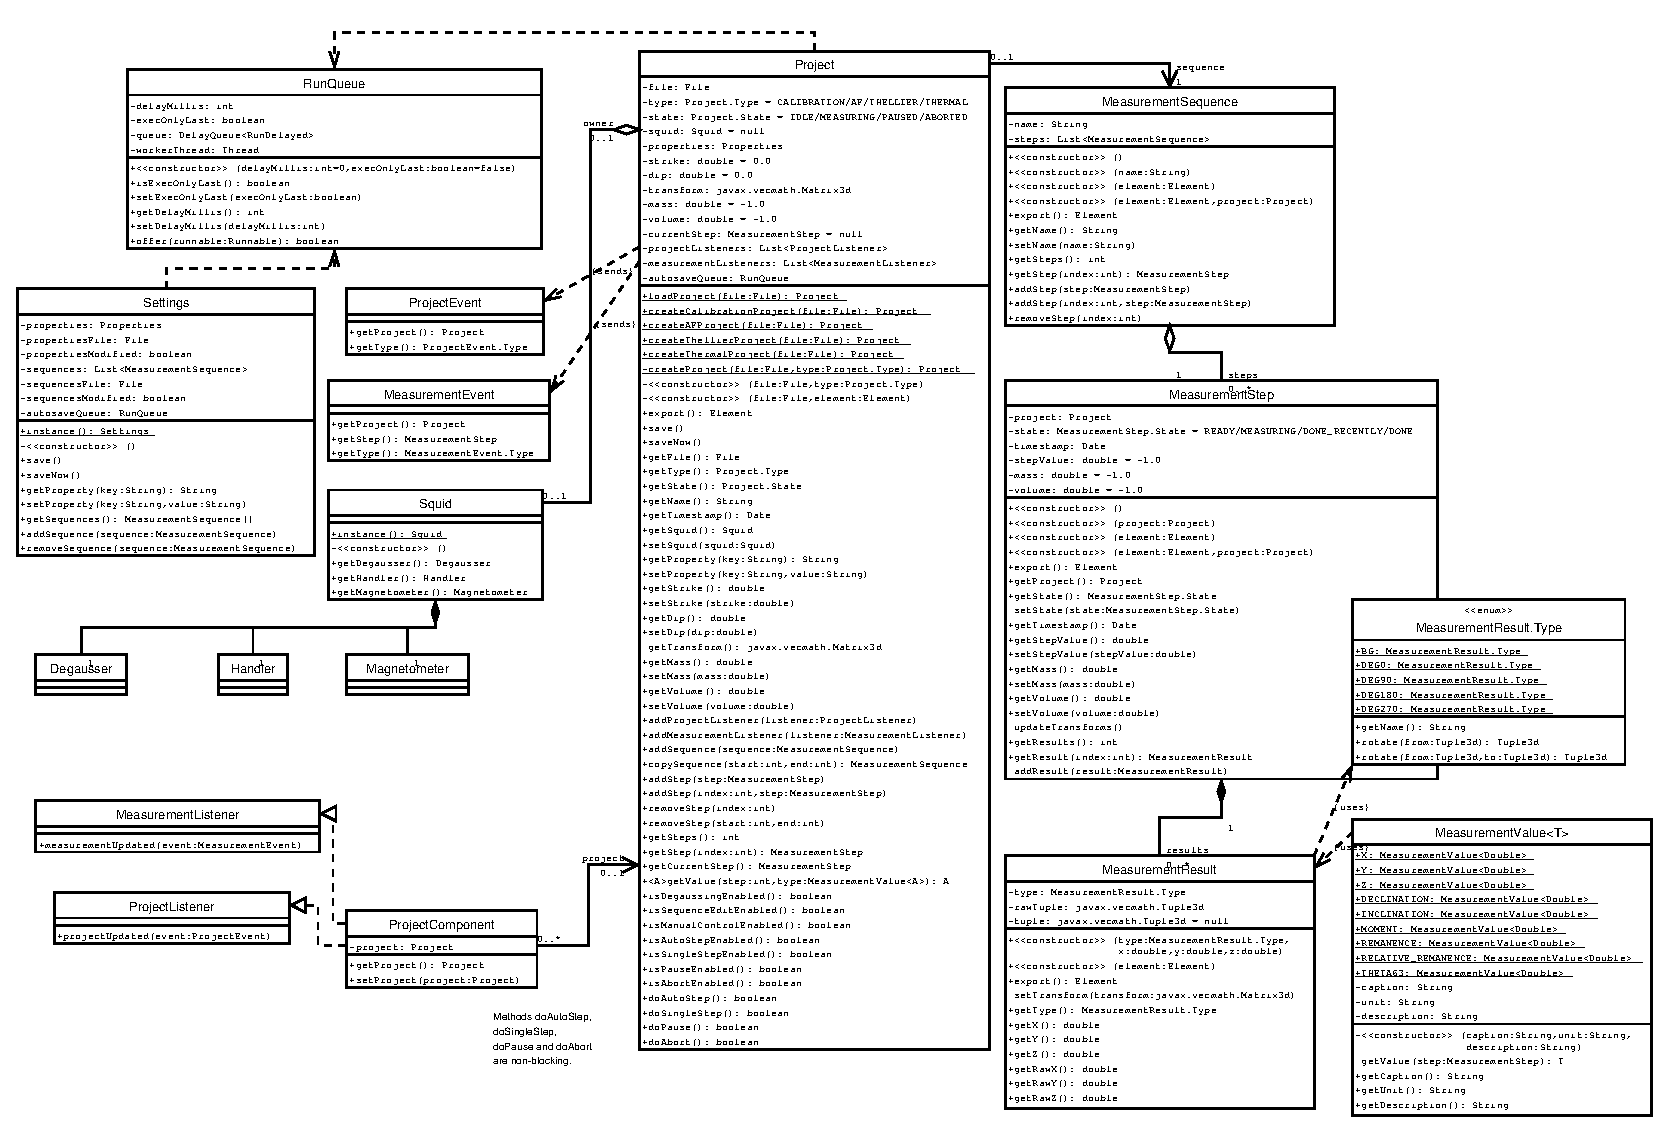
\includegraphics[angle=90,width=14cm]{class-diagram-part1.eps}
\caption{Squid class diagram: central classes}
\label{fig:classdiagram1}
\end{center}
\end{figure}

\begin{figure}
\begin{center}
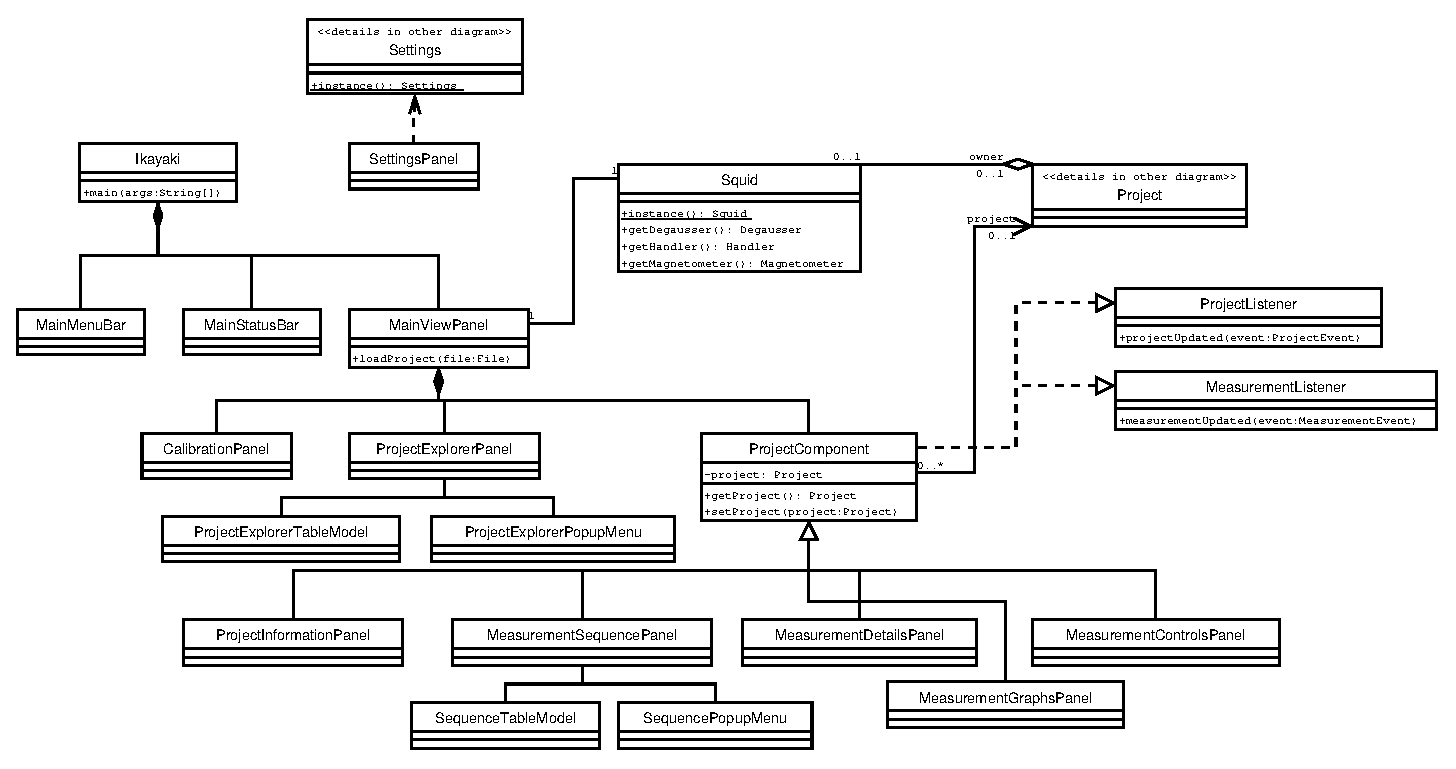
\includegraphics[angle=90,width=14cm]{class-diagram-part2.eps}
\caption{Squid class diagram: GUI classes}
\label{fig:classdiagram2}
\end{center}
\end{figure}

See Figure~\ref{fig:classdiagram1} and Figure~\ref{fig:classdiagram2}.


\section{Architecture description}


\section{Classes and methods}


\subsection{Main view and menu}


\subsection{Configuration window}


\subsection{Project Explorer}


\beginClass{ProjectExplorerPanel}
\classPackage{ikayaki.gui}
\classDeclaration{public class ProjectExplorerPanel}
\classExtends{JPanel}
\classCreatedBy{MainViewPanel}
\classUses{ProjectExplorerTableModel}
\classUses{ProjectExplorerPopupMenu}
\classComment{
	Creates a history/autocomplete field (browserField) for choosing the project directory, a listing of project files in that directory (explorerTable) and in that listing a line for creating new project, which has a textbox for project name, an AF/TH ComboBox and a "Create new" button for actuating the creation. Also has a right-click popup menu for exporting project files.
}
\classEvent{On browserField change}{send browserField's text to RunQueue which schedules disk access and autocomplete. (This could be in a separate BrowserFieldComponent class)}
\classEvent{On explorerTable mouse right-click}{create a ProjectExplorerPopupMenu for right-clicked project file. (This could be in ProjectExplorerTableModel class)}
\classEvent{On createNewProject mouseclick}{create a new project, set it active and tell ProjectExplorerTableMode to update itself.}
\classEvent{On browseButton mouseclick}{open a FileChooser dialog for choosing the directory.}
\closeClass

\beginField{browserField}
\fieldDeclaration{private BrowserFieldComponent browserField}
\fieldComment{
(need a separate class for this?)
}
\closeField

\beginField{explorerTable}
\fieldDeclaration{private ProjectExplorerTableModel explorerTable}
\closeField

\beginField{createNewProject}
\fieldDeclaration{private JButton createNewProject}
\closeField

\beginField{browseButton}
\fieldDeclaration{private JButton browseButton}
\closeField

\beginField{newProject}
\fieldDeclaration{private JTextField newProject}
\closeField

\beginField{JComboBox newProjectType}
\fieldDeclaration{private JComboBox newProjectType}
\closeField

\beginMethod{ProjectExplorerPanel()}
\methodDeclaration{public ProjectExplorerPanel()}
\methodComment{
	Creates its components, places them and sets the last project folder as current project folder.
}
\closeMethod

\beginMethod{createNewProject()}
\methodDeclaration{public void createNewProject()}
\methodComment{
	Creates a new project, sets it active, sends it to MainViewPanel, tells explorerTable to reset newProject and newProjectType fields.
}
\closeMethod

\beginMethod{doBrowse()}
\methodDeclaration{public void doBrowse()}
\methodComment{
	Creates a FileChooser dialog and tells explorerTable and browserField to change to directory returned by it.
}
\closeMethod


\beginClass{ProjectExplorerTableModel}
\classPackage{ikayaki.gui}
\classDeclaration{public class ProjectExplorerTableModel}
\classExtends{AbstractTableModel}
\classCreatedBy{ProjectExplorerPanel}
\classUses{MainViewPanel}
\classComment{
	Creates a list of project files in directory. Handles loading selected projects and executing export choice.
}
\classEvent{On newDirectoryEvent}{updates list of project files on JTable}
\classEvent{On selectTable MouseEvent}{sets new Project active}
\closeClass

\beginField{directory}
\fieldDeclaration{private File directory}
\fieldValue{null}
\fieldComment{
	Currently opened directory
}
\closeField

\beginField{files}
\fieldDeclaration{private Vector<File> files}
\fieldValue{new Vector<File>()}
\fieldComment{
	Project files in the current directory.
}
\closeField

\beginMethod{ProjectExplorerTableModel()}
\methodDeclaration{public ProjectExplorerTableModel()}
\methodComment{
	Reads the contents of the default directory and initializes the file list.
}
\closeMethod

\beginMethod{ProjectExplorerTableModel(String)}
\methodDeclaration{public ProjectExplorerTableModel(String directory)}
\methodComment{
	Reads the contents of the given directory and initializes the file list.
}
\methodParam{directory}{path to the directory to be opened}
\closeMethod

\beginMethod{loadDirectory(String)}
\methodDeclaration{public void loadDirectory(String directory)}
\methodComment{
	Update list to show given directory.
}
\methodParam{directory}{path to the directory to be opened}
\closeMethod

\beginMethod{loadProject()}
\methodDeclaration{public void loadProject()}
\methodComment{
	Gets the selected line from the file list and sends the file to MainViewPanel.
}
\closeMethod


\beginClass{ProjectExplorerPopupMenu}
\classPackage{ikayaki.gui}
\classDeclaration{public class ProjectExplorerPopupMenu}
\classExtends{JPopupMenu}
\classCreatedBy{ProjectExplorerPanel}
\classComment{
	Shows choices to export: AF, Thellier, Thermal and executes selected
}
\classEvent{On selectItem mouseEvent}{tells selected Project to create selected file from it's self}
\closeClass

\beginMethod{ProjectExplorerTableModel()}
\methodDeclaration{public ProjectExplorerTableModel()}
\methodComment{
	Builds the menu items
}
\closeMethod

\beginClass{MainViewPanel}
\classPackage{ikayaki.gui}
\classDeclaration{public class MainViewPanel}
\classExtends{JPanel}
\classCreatedBy{Ikayaki}
\classUses{ProjectExplorerPanel}
\classUses{CalibrationPanel}
\classUses{Squid}
\classUses{MainMenuBar}
\classUses{MainStatusBar}
\classUses{ProjectInformationPanel}
\classUses{MeasurementSequencePanel}
\classUses{MeasurementDetailsPanel}
\classUses{MeasurementControlsPanel}
\classUses{MeasurementGraphsPanel}
\classComment{
    Creates the main view panels (split panels) and Squid and Project components. It also tells everybody if project file is changed. 
}
\closeClass

\beginField{projectExplorer}
\fieldDeclaration{private ProjectExplorerPanel projectExplorer}
\closeField

\beginField{calibration}
\fieldDeclaration{private CalibrationPanel calibration}
\closeField

\beginField{squid}
\fieldDeclaration{private Squid squid}
\closeField

\beginField{project}
\fieldDeclaration{private ProjectComponent project}
\fieldComment{currently active project}
\closeField

\beginField{menuBar}
\fieldDeclaration{private MainMenuBar menuBar}
\closeField

\beginField{statusBar}
\fieldDeclaration{private MainStatusBar statusBar}
\closeField

\beginField{projectInformation}
\fieldDeclaration{private ProjectInformationPanel projectInformation}
\closeField

\beginField{measurementSequence}
\fieldDeclaration{private MeasurementSequencePanel measurementSequence}
\closeField

\beginField{measurementControls}
\fieldDeclaration{private MeasurementControlsPanel measurementControls}
\closeField

\beginField{measurementDetails}
\fieldDeclaration{private MeasurementDetailsPanel measurementDetails}
\closeField

\beginField{measurementGraphs}
\fieldDeclaration{private MeasurementGraphsPanel measurementGraphs}
\closeField

\beginMethod{MainViewPanel()}
\methodDeclaration{public MainViewPanel()}
\methodComment{
    Loads default view and creates all components and panels. Splitpanel between Calibration,Explorer,Information and rest.
}
\closeMethod

\beginMethod{changeProject(String filename)}
\methodDeclaration{public bool changeProject(String filename)}
\methodComment{
    Looks for file with filename, if not exist creates new other wise opens it. Then updates current project and tells Panels new project is opened.
}
\closeMethod


\beginClass{MainMenuBar}
\classPackage{ikayaki.gui}
\classDeclaration{public class MainMenuBar}
\classExtends{JMenuBar}
\classCreatedBy{MainViewPanel}
\classComment{Creates Menu items for Menubar and makes action listeners for them}

\classEvent{On newProject Clicked}{Opens File chooser and opens new file in selected folder}
\classEvent{On openProject Clicked}{Opens File chooser and opens selected file}
\classEvent{On exportToDAT Clicked}{Opens File chooser and tells Project to export in selected file}
\classEvent{On exportToDTDT Clicked}{Opens File chooser and tells Project to export in selected file}
\classEvent{On exportToSRM Clicked}{Opens File chooser and tells Project to export in selected file}
\classEvent{On configuration Clicked}{Opens SettingsPanel (frame)}
\classEvent{On helpItem Clicked}{Opens Help dialog (own frame?)}
\classEvent{On about Clicked}{Opens dialog with credits and version number}
\classEvent{On exit Clicked}{closes program}

\closeClass

\beginField{file}
\fieldDeclaration{private JMenu file}
\closeField

\beginField{options}
\fieldDeclaration{private JMenu options}
\closeField

\beginField{help}
\fieldDeclaration{private JMenu help}
\closeField

\beginField{newProject}
\fieldDeclaration{private JMenuItem newProject}
\closeField

\beginField{openProject}
\fieldDeclaration{private JMenuItem openProject}
\closeField

\beginField{exportProject}
\fieldDeclaration{private JMenu exportProject}
\closeField

\beginField{exportProjectToDAT}
\fieldDeclaration{private JMenuItem exportProjectToDAT}
\closeField

\beginField{exportProjectToTDT}
\fieldDeclaration{private JMenuItem exportProjectToDTD}
\closeField

\beginField{exportProjectToSRM}
\fieldDeclaration{private JMenuItem exportProjectToSRM}
\closeField

\beginField{exit}
\fieldDeclaration{private JMenuItem exit}
\closeField

\beginField{configuration}
\fieldDeclaration{private JMenuItem configuration}
\closeField

\beginField{helpItem}
\fieldDeclaration{private JMenuItem helpItem}
\closeField

\beginField{about}
\fieldDeclaration{private JMenuItem about}
\closeField

\beginMethod{MainMenuBar()}
\methodDeclaration{public MainMenuBar()}
\methodComment{
    Creates all components and makes menu and sets ActionListeners.
}
\closeMethod

\beginClass{MainStatusBar}
\classPackage{ikayaki.gui}
\classDeclaration{public class MainStatusBar}
\classExtends{ProjectComponent}
\classCreatedBy{MainViewPanel}
\classComment{Creates its components and listens project events on status change and calculates estimated time for measurement}

\classEvent{On Measurement Event}{recalculates progress and updates status for current measurement}
\closeClass

\beginField{measurementStatus}
\fieldDeclaration{private JLabel measurementStatus}
\fieldComment{text comment of current status(moving,measurement,demagnetization)}
\closeField

\beginField{measurementProgress}
\fieldDeclaration{private JProgressBar measurementProgress}
\fieldComment{progress of sequence/measurement as per cent of whole process}
\closeField

\beginField{currentSequence}
\fieldDeclaration{private int[] currentSequence}
\fieldComment{current projects sequence}
\closeField

\beginField{projectType}
\fieldDeclaration{private int projectType}
\fieldComment{current projects type (we know if we are doing demagnetization or not)}
\closeField

\beginMethod{MainStatusBar()}
\methodDeclaration{public MainStatusBar()}
\methodComment{
    Creates all components with default settings and sets Listener for MeasurementEvent.
}
\closeMethod

\beginMethod{calculateStatus(int sequenceStep,int currentStep)}
\methodDeclaration{private void calculateStatus(String phase,int sequenceStep,int currentStep)}
\methodComment{
    Recalculates current progress and updates status.
}
\closeMethod

\beginMethod{setMeasurement(int projectType,int[] sequence)}
\methodDeclaration{{private void setMeasurement(int projectType,int[] sequence)}
\methodComment{
    Formats status and creates new measurement status values.
}
\closeMethod

\beginClass{SettingsPanel}
\classPackage{ikayaki.gui}
\classDeclaration{public class SettingsPanel}
\classExtends{JFrame}
\classCreatedBy{MainStatusBar}
\classUses{Settings}
\classComment{Creates its components and updats changes to Settings and saves them in Configuration file}

\classEvent{On Save Clicked}{saves current configuration to Settings-singleton and closes window}
\classEvent{On Cancel Clicked}{closes window (discarding changes)}

\closeClass

\beginField{magnetometerPort}
\fieldDeclaration{private JComboBox magnetometerPort}
\fieldComment{COM port for magnetometer}
\closeField

\beginField{demagnetizerPort}
\fieldDeclaration{private JComboBox demagnetizerPort}
\fieldComment{COM port for demagnetizer, can be sharing same port with magnetometer}
\closeField

\beginField{handlerPort}
\fieldDeclaration{private JComboBox handlerPort}
\fieldComment{COM port for sample handler}
\closeField

\beginField{xAxisCalibration}
\fieldDeclaration{private JTextField xAxisCalibration}
\fieldComment{Calibration constants with polarization (factory set?)}
\closeField

\beginField{yAxisCalibration}
\fieldDeclaration{private JTextField yAxisCalibration}
\fieldComment{Calibration constants with polarization (factory set?)}
\closeField

\beginField{zAxisCalibration}
\fieldDeclaration{private JTextField zAxisCalibration}
\fieldComment{Calibration constants with polarization (factory set?)}
\closeField

\beginField{demagRamp}
\fieldDeclaration{private JComboBox demagRamp}
\fieldComment{how fast demagnetization goes}
\closeField

\beginField{demagDelay}
\fieldDeclaration{private JComboBox demagDelay}
\fieldComment{?}
\closeField

\beginField{acceleration}
\fieldDeclaration{private JTextField acceleration}
\fieldComment{Handler acceleration}
\closeField

\beginField{deceleration}
\fieldDeclaration{private JTextField deceleration}
\fieldComment{Handler deceleration}
\closeField

\beginField{velocity}
\fieldDeclaration{private JTextField velocity}
\fieldComment{Handler Max speed}
\closeField

\beginField{measurementVelocity}
\fieldDeclaration{private JTextField measurementVelocity}
\fieldComment{speed in measurement, should be small}
\closeField

\beginField{transverseYPosition}
\fieldDeclaration{private JTextField transverseYPosition}
\closeField

\beginField{axialPosition}
\fieldDeclaration{private JTextField axialPosition}
\closeField

\beginField{sampleLoadPosition}
\fieldDeclaration{private JTextField sampleLoadPosition}
\closeField

\beginField{backgroundPosition}
\fieldDeclaration{private JTextField backgroundPosition}
\closeField

\beginField{measurementPosition}
\fieldDeclaration{private JTextField measurementPosition}
\closeField

\beginField{rotation}
\fieldDeclaration{private JTextField rotation}
\closeField

\beginField{handlerRightLimit}
\fieldDeclaration{private JComboBox handlerRightLimit}
\closeField

\beginField{saveButton}
\fieldDeclaration{private JButton saveButton}
\closeField

\beginField{cancelButton}
\fieldDeclaration{private JButton cancelButton}
\closeField


\beginMethod{SettingsPanel()}
\methodDeclaration{public SettingsPanel()}
\methodComment{
    Creates all components and puts them in right places. Labels are created only here (no global fields). Creates ActionListeners for buttons.
}
\closeMethod

\beginMethod{closeWindow()}
\methodDeclaration{public void closeWindow()}
\methodComment{
    Closes window, no changes saved.
}
\closeMethod

\beginMethod{saveSettings()}
\methodDeclaration{public void saveSettings()}
\methodComment{
    Saves all settings to Settings-singleton and calls closeWindow().
}
\closeMethod


\subsection{Calibration}


\subsection{Project information}


\subsection{Project file}


\subsection{Sequence and measurement data}


\subsection{Measurement details}


\subsection{Measurement controls}

\beginClass{MeasurementControlsPanel}
\classPackage{ikayaki.gui}
\classDeclaration{public class MeasurementControlsPanel}
\classExtends{ProjectComponent}
\classCreatedBy{MainViewPanel}
\classUses{Project}
\classUses{MagnetometerStatusPanel}
\classUses{ManualControlsPanel}
\classComment{
	Has "Measure"/"Pause", "Single step" and "Stop now!" buttons for controlling measurements; "+z/-z" radiobuttons for changing sample orientation, help picture for inserting sample, picture of current magnetometer status, and, manual controls.
	Listens MeasurementEvents and ProjectEvents, and updates buttons and magnetometer status accordingly.
}
\classEvent{On measureButton click}{call project.doAutoStep() or project.doPause(), depending on current button status.}
\classEvent{On singlestepButton click}{call project.doSingleStep().}
\classEvent{On stopButton click}{call project.doAbort().}
\classEvent{On MeasurementEvent}{call magnetometerStatusPanel.updateStatus(int, int).}
\classEvent{On ProjectEvent}{update buttons and manual controls according to project.isXXXEnabled().}
\closeClass

\beginField{project}
\fieldDeclaration{private Project project}
\closeField

\beginField{measureButton}
\fieldDeclaration{private JButton measureButton}
\closeField

\beginField{singlestepButton}
\fieldDeclaration{private JButton singlestepButton}
\closeField

\beginField{stopButton}
\fieldDeclaration{private JButton stopButton}
\closeField

\beginField{zPlusRadioButton}
\fieldDeclaration{private JRadioButton zPlusRadioButton}
\closeField

\beginField{zMinusRadioButton}
\fieldDeclaration{private JRadioButton zMinusRadioButton}
\closeField

\beginField{sampleInsertImage}
\fieldDeclaration{private JImage? sampleInsertImage}
\closeField

\beginField{magnetometerStatusPanel}
\fieldDeclaration{private MagnetometerStatusPanel magnetometerStatusPanel}
\closeField

\beginField{manualControlsPanel}
\fieldDeclaration{private ManualControlsPanel manualControlsPanel}
\closeField

\beginClass{MagnetometerStatusPanel}
\classPackage{ikayaki.gui}
\classDeclaration{public class MagnetometerStatusPanel}
\classExtends{JPanel}
\classCreatedBy{MeasurementControlsPanel}
\classComment{Picture of current magnetometer status, including sample holder position and rotation.}
\closeClass

\beginMethod{updateStatus(int, int)}
\methodDeclaration{public updateStatus(int position, int rotation)}
\methodComment{Updates magnetometer status picture; called by MeasurementControlsPanel.}
\methodParam{position}{sample holder position, from a to b?}
\methodParam{rotation}{sample holder rotation; 0, 90, 180 or 270.}
\closeMethod

\beginClass{ManualControlsPanel}
\classPackage{ikayaki.gui}
\classDeclaration{public class ManualControlsPanel}
\classExtends{JPanel}
\classCreatedBy{MeasurementControlsPanel}
\classComment{Magnetometer manual control radiobuttons.}
\classUses{Project}
\classEvent{On xxxN click}{call project.xxxN().}
\closeClass

\beginField{project}
\fieldDeclaration{private Project project}
\closeField

\beginField{demagX}
\fieldDeclaration{private JRadioButton demagX}
\closeField

\beginField{demagY}
\fieldDeclaration{private JRadioButton demagY}
\closeField

\beginField{demagZ}
\fieldDeclaration{private JRadioButton demagZ}
\closeField

\beginField{measureX}
\fieldDeclaration{private JRadioButton measureX}
\closeField

\beginField{measureY}
\fieldDeclaration{private JRadioButton measureY}
\closeField

\beginField{measureZ}
\fieldDeclaration{private JRadioButton measureZ}
\closeField


\subsection{Status bar}


\subsection{Graphs}


\subsection{Squid interface}


\subsection{Serial communication interface}


\subsection{Squid emulator}


\subsection{Utilities}


\beginClass{RunQueue}
\classPackage{ikayaki.util}
\classDeclaration{public class RunQueue}
\classUses{RunQueue.RunQueueThread}
\classUses{RunQueue.RunDelayed}
\classComment{
	Executes Runnable objects in a private worker thread after a pre-defined delay. The worker thread will terminate automatically when there are no runnables to be executed. Optionally executes only the last inserted runnable. All operations are thread-safe.

	This class can be used for example in connection with a "continuous search" invoked by a series of GUI events (such as a DocumentListener), but it is necessary to react to only the last event after a short period of user inactivity.
}
\classPatterns{Command}
\closeClass

\beginField{delayMillis}
\fieldDeclaration{private int delayMillis}
\fieldValue{0}
\fieldComment{
	Defines how long is the delay in milliseconds, after which the events need to be run.
}
\closeField

\beginField{execOnlyLast}
\fieldDeclaration{private boolean execOnlyLast}
\fieldValue{false}
\fieldComment{
	Defines if only the last event should be executed. If false, then all of the events are executed in the order of appearance.
}
\closeField

\beginField{queue}
\fieldDeclaration{private DelayQueue<RunDelayed> queue}
\fieldValue{new DelayQueue<RunDelayed>()}
\fieldComment{
	Prioritized FIFO queue for containing the RunDelayed items that have not expired. If execOnlyLast is true, then this queue should never contain more than one item.
}
\closeField

\beginField{workerThread}
\fieldDeclaration{private Thread workerThread}
\fieldValue{null}
\fieldComment{
	The worker thread that will run the inserted runnables. If the thread has no more work to do, it will set workerThread to null and terminate itself.
}
\closeField

\beginMethod{RunQueue()}
\methodDeclaration{public RunQueue()}
\methodComment{
	Creates an empty RunQueue with a delay of 0 and execOnlyLast set to false.
}
\closeMethod

\beginMethod{RunQueue(int)}
\methodDeclaration{public RunQueue(int delayMillis)}
\methodComment{
	Creates an empty RunQueue with execOnlyLast set to false.
}
\methodParam{delayMillis}{the length of execution delay in milliseconds; if less than 0, then 0 will be used.}
\closeMethod

\beginMethod{RunQueue(boolean)}
\methodDeclaration{public RunQueue(boolean execOnlyLast)}
\methodComment{
	Creates an empty RunQueue with a delay of 0.
}
\methodParam{execOnlyLast}{if true, only the last event will be executed after the delay; otherwise all are executed in order of appearance.}
\closeMethod

\beginMethod{RunQueue(int,boolean)}
\methodDeclaration{public RunQueue(int delayMillis, boolean execOnlyLast)}
\methodComment{
	Creates an empty RunQueue.
}
\methodParam{delayMillis}{the length of execution delay in milliseconds; if less than 0, then 0 will be used.}
\methodParam{execOnlyLast}{if true, only the last event will be executed after the delay; otherwise all are executed in order of appearance.}
\closeMethod

\beginMethod{isExecOnlyLast()}
\methodDeclaration{public synchronized boolean isExecOnlyLast()}
\methodReturn{true if only the last event will be executed after the delay; otherwise false.}
\closeMethod

\beginMethod{setExecOnlyLast(boolean)}
\methodDeclaration{public synchronized void setExecOnlyLast(boolean execOnlyLast)}
\methodParam{execOnlyLast}{if true, only the last event will be executed after the delay; otherwise all are executed in order of appearance.}
\closeMethod

\beginMethod{getDelayMillis()}
\methodDeclaration{public synchronized int getDelayMillis()}
\methodReturn{the delay in milliseconds}
\closeMethod

\beginMethod{setDelayMillis(int)}
\methodDeclaration{public synchronized void setDelayMillis(int delayMillis)}
\methodParam{delayMillis}{delay in milliseconds; if less than 0, then the new value is ignored.}
\closeMethod

\beginMethod{offer(Runnable)}
\methodDeclaration{public synchronized boolean offer(Runnable runnable)}
\methodComment{
	Inserts a Runnable object to the end of the queue. It will remain there until it is executed or another object replaces it. If execOnlyLast is set to true, the queue will be cleared before inserting this runnable to it. If there is no worker thread running, a new one will be spawned.
}
\methodParam{runnable}{the Runnable to be run after a pre-defined delay}
\methodReturn{true}
\methodThrows{NullPointerException}{if runnable is null}
\closeMethod


\beginClass{RunQueue.RunQueueThread}
\classPackage{ikayaki.util}
\classDeclaration{private class RunQueueThread}
\classExtends{Thread}
\classCreatedBy{RunQueue}
\classComment{
	Keeps on checking the RunQueue.queue to see if there are Runnables to be executed. If there is one, execute it and proceed to the next one. If an uncaught Throwable is thrown during the execution, prints an error message and stack trace to stderr. If the queue is empty, this thread will set RunDelayed.workerThread to null and terminate itself.
}
\closeClass

\beginMethod{run()}
\methodDeclaration{public void run()}
\closeMethod


\beginClass{RunQueue.RunDelayed}
\classPackage{ikayaki.util}
\classDeclaration{private class RunDelayed}
\classImplements{Delayed}
\classCreatedBy{RunQueue}
\classComment{	
	Wraps a Runnable object and sets the delay after which it should be executed by a worker thread.
}
\closeClass

\beginField{expires}
\fieldDeclaration{private long expires}
\fieldComment{
	The point in time when this RunDelayed will expire.
}
\closeField

\beginField{runnable}
\fieldDeclaration{private Runnable runnable}
\fieldComment{
	Contained Runnable object to be run after this RunDelayed has expired.
}
\closeField

\beginMethod{RunDelayed(Runnable,int)}
\methodDeclaration{public RunDelayed(Runnable runnable, int delayMillis)}
\methodComment{
	Creates a new RunDelayed item that contains runnable.
}
\methodParam{runnable}{the Runnable to be contained}
\methodParam{delayMillis}{delay in milliseconds}
\closeMethod

\beginMethod{getDelay(TimeUnit)}
\methodDeclaration{public long getDelay(TimeUnit unit)}
\methodComment{
	Returns the remaining delay associated with this object, always in milliseconds.
}
\methodParam{unit}{ignored; always assumed TimeUnit.MILLISECONDS}
\methodReturn{the remaining delay; zero or negative values indicate that the delay has already elapsed}
\closeMethod

\beginMethod{getRunnable()}
\methodDeclaration{public Runnable getRunnable()}
\methodComment{
	Returns the contained Runnable.
}
\methodReturn{the Runnable given as constructor parameter}
\closeMethod

\beginMethod{compareTo(Delayed)}
\methodDeclaration{public int compareTo(Delayed delayed)}
\methodComment{
	Compares this object with the specified object for order.  Returns a negative integer, zero, or a positive integer as this object is less than, equal to, or greater than the specified object.
}
\methodParam{delayed}{the Delayed to be compared.}
\methodReturn{a negative integer, zero, or a positive integer as this delay is less than, equal to, or greater than the specified delay.}
\closeMethod


\section{Package structure}

\section{Bibliography}
